\documentclass[12pt]{article}
\usepackage[margin=1in]{geometry}
\usepackage{amsmath}
\usepackage{amssymb}
\usepackage{setspace}
\usepackage{graphicx}
\usepackage{cite}

\title{Natural Computing Assessment}
\author{Exam Nos. B156771, [insert exam number here]}

\begin{document}
\maketitle
\section{Neural Network Training with PSO}
\subsection{Choosing the Fitness Function}
This task is interpreted to mean that we are to design a fitness function to evaluate the fitness of the network as a whole after it has been trained, as to use the testing error for optimisation of the model itself contradicts the idea of a test set.
Let the training error $e_T$, and the testing error $e_\tau$. 
Taking the average of the two would be a sensible, if not standard course of action. 
However, a fitness function would need to incorporate a measure of how overfit the model is to the training data in order to be effective. 
In this sense, adding the difference between the two values is simple and effective. 
Ultimately, the fitness function takes the following form:
\begin{equation}
    f(e_T, e_\tau) = 1 - \left(\frac{e_T + e_\tau}{2} + \left(e_\tau - e_T\right)\right),
\end{equation}
where the error is calculated using the Mean Squared Error function. We subtract the average and distance from 1 to ensure that a greater fitness value implies a better model.

\subsection{Defining the Search Space}
The search space of a PSO is given by $[a,b]^D$, where $a,b\in \mathbb{R}$, and $D\in\mathbb{N}$ is the dimension of the space. 
We define the shape of a neural network by a sequence $(a_n)_{n=1}^{l}$ where $l\in\mathbb{N}$ defines the number of layers, and each $a_n \in \mathbb{N}$ gives the number of neurons in layer $n$. 
The dimension of the weight vector for a would be the number of edges connecting each sequential pair of layers, plus the biases, given by the number of neurons in the latter of the pair of layers. Succinctly, the dimension $D$ of the search space is given by,
\begin{equation}
    D = \left(\sum_{i=1}^{l-1} a_{n+1}\left(a_n + 1\right)\right) - a_l,
\end{equation}
where the final decrement addresses non-existent bias terms in the output layer that were counted in the summation.

For this task, we set the shape to be $\left(4, 8, 1\right)$, meaning that the dimension of the search space $D=43$. 
To ensure that we are notified of a divergent swarm, we set $-a=b=20$, meaning that the search space for the PSO will be $\left[-20,20\right]^{43}$. 

\subsection{Training the Model}
For this task we trained two neural networks: one using Particle Swarm as its optimiser, and another using Stochastic Gradient Descent.
The model using SGD provides a fairly standard baseline on which to test the PSO model. 
In the code provided, the PSO neural net does not use any third party machine learning libraries as due to the nature of PSO, these neural nets only needed to consider forward propagation, not backwards.
For the SGD optimised net, Pytorch was used due to the myriad of material online explaining how to code it. 

Each network was trained with 2-fold cross validation using the cross-validate program provided (refer to the README in the task-1 directory on how to use it). 
Two folds was chosen to adhere more closely to the instructions in the assignment, where half of the entire data set was used for training, and the other for testing.
The parameters for the PSO were as follows: $n=20$, $\omega=0.7$, $\alpha_1 = 1.5 \alpha_2 = 1.3$. 
The parameters for the SGD were as follows: learning rate $=0.03$.
The figure below shows the training and testing loss of both over time:

\begin{figure}[h]                   
      \begin{center}                  
          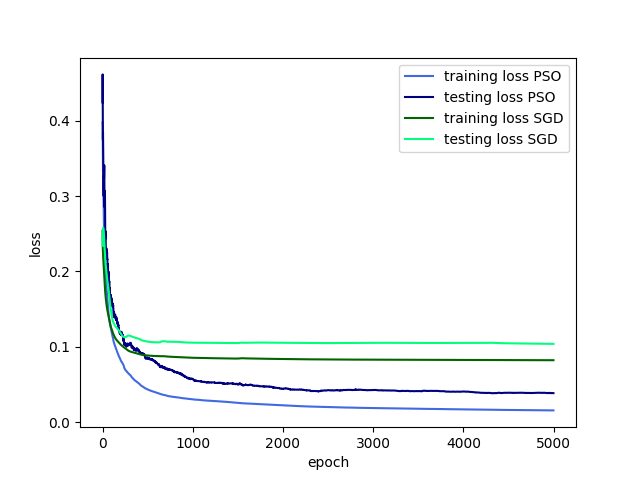
\includegraphics[scale=0.45]{/home/alexander/school/natural_computing/task-1/data/figures/nonlinear.png}    
      \end{center}                                                                                              
\end{figure}
The table below shows the final average training and testing losses, as well as the average fitness using equation (1):
\begin{center}
 \begin{tabular}{||c c c c||} 
 \hline
 Optimiser & Average Training Loss & Average Testing Loss & Average Fitness \\ [0.5ex] 
 \hline\hline
 PSO & 0.0102 & 0.024 & 0.969 \\ 
 \hline
 SGD & 0.0444 & 0.0549 & 0.939 \\
 \hline
\end{tabular}
\end{center}

By these results it would appear that the model trained using PSO as its optimiser performed significantly better than the model trained with SGD. 
In a way, this could almost be expected. Gradient Descent follows the single path of a point gradually moving along the steepest descent in the search space.
In contrast, Particle Swarm has several particles searching for the (ideally) global, if not various local minima. 
This means that PSO is more likely to find a global minimum than SGD is, though how much more likely is still to be determined.
Nevertheless, it is clear that for our purposes the PSO is superior. 
While it was slower to train, the low loss on both the training and testing sets for each fold of the cross validation demonstrates that it is well suited for neural network training. Furthermore, by eliminating backpropagation as a consideration in training, developing the model is conceptually simpler as well. 
\subsection{Restriction to Linear Inputs}
Imposing a restriction to linear inputs, we decided to change the architecture of the models. 
For this part of the task, the models shape will be $(2, 6, 5, 1)$.
This yielded the following results:
\begin{figure}[h]                   
      \begin{center}                  
          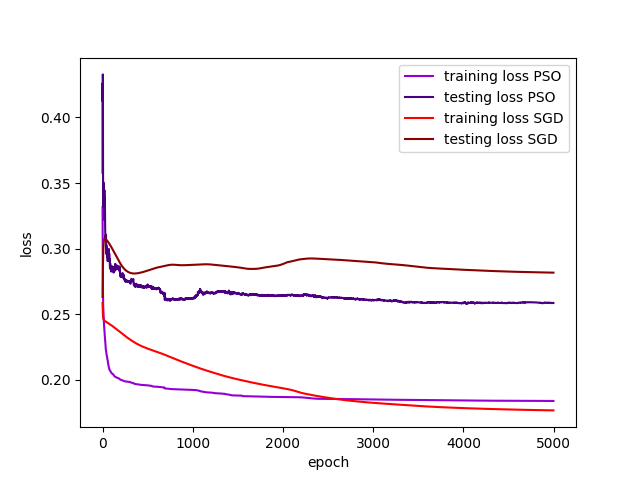
\includegraphics[scale=0.45]{../task-1/data/figures/linear.png}    
      \end{center}                                                                                              
\end{figure}
\begin{center}
 \begin{tabular}{||c c c c||} 
 \hline
 Optimiser & Average Training Loss & Average Testing Loss & Average Fitness \\ [0.5ex] 
 \hline\hline
 PSO & 0.0657 & 0.1248 & 0.1574 \\ 
 \hline
 SGD & 0.1639 & 0.2654 & 0.3162 \\
 \hline
\end{tabular}
\end{center}

The restriction to linear inputs was clearly a terrible idea.
These models performed significantly worse in all aspects when compared to their nonlinear counterparts, which is to be expected. Linear inputs do not lend themselves well to the curvature of the spiral dataset. 
By allowing nonlinear transformations to the data point, we are able to introduce curved aspects to the output space which is able to better fit the data.  
\subsection{The Effect of Particle Swarm Parameters}
For this part of the task, we took a look at how changing various parameters affected the final training and testing errors, as well as the overall fitness of the model.
First, we took a look at varying $\omega$, considering $\omega = \{0.1, 0.2, \ldots, 0.9\}$. The table showing these results is in the appendix. 
Here it is helpful to remember that $\omega$ indicates what percentage of the previous iteration's velocity is still present in the particle. Too little and the particles would have trouble moving, being guided primarily by the personal and global bests. Too much and the particle would have a hard time changing direction when the swarm dictates it to. One would expect the optimal $\omega$ to be somewhere near the middle then, and indeed our results show that the best $\omega = 0.7$, earning the network a fitness of 0.9208. 

While $\omega$ concerns itself with the velocity term, the parameters $\alpha_1$ and $\alpha_2$ help determine the weight of the personal and global bests in comparison to the particles current position.
We ran a similar experiment varying the value of $\alpha$ between 1.2 and 2.1. We decided for the sake of simplicity to follow convention and keep $\alpha_1=\alpha_2$. The table with this data is also in the appendix.

Observe that the difference between the fitness of each model as we change the $\alpha$ parameter is much smaller than when we changed $\omega$. More notable; however, is that while changes in $\omega$ appeared to provide a smoother change in the fitness, changes in the $\alpha$ term do not, meaning that it would be much harder to choose properly. It stands to reason that the higher the value of $\alpha$, the more volatile the particle's movements will be, unless the particle is close to the optimal position. So a higher $\alpha$ would allow the possibility for a particle to overshoot the optimal position. In contrast, too low an $\alpha$ and the particle would be guided only by its intertia. Again, logically the best place to start looking then would be a median point between the two extremes. The table in appendix A shows that the $\alpha$ value with the best fitness is $\alpha=1.5$, which does fit with our hypothesis. This, of course, is a heuristic for where to start looking rather than a definitive guide. From this, one could draw the conclusion that extreme values for these parameters would almost never provide an optimal solution, and that it would be better to start with a more middle value for each and adjust accordingly (or even better, use a MHO algorithm to find the optimal parameters).

\appendix
\section{Tables and Figures}
Results of experiments with varying $\omega$ ($\alpha_1=\alpha_2=1.6$):
\begin{center}
 \begin{tabular}{||c c c c||} 
 \hline
 $\omega$ & $e_T$ & $e_\tau$ & $f$ \\ [0.5ex] 
 \hline\hline
 0.1 & 0.2372 & 0.2975 & 0.6723 \\ 
 \hline
 0.2 & 0.1946 & 0.2733 & 0.6873 \\
 \hline
 0.3 & 0.1467 & 0.195 & 0.7808 \\
 \hline
 0.4 & 0.1823 & 0.252 & 0.7131 \\
 \hline
 0.5 & 0.0928 & 0.1714 & 0.7893 \\
 \hline
 0.6 & 0.0129 & 0.0629 & 0.9121 \\
 \hline
 0.7 & 0.0097 & 0.056 & 0.9208 \\
 \hline
 0.8 & 0.1976 & 0.2541 & 0.7176 \\
 \hline
 0.9 & 0.4023 & 0.2909 & 0.542 \\
 \hline
\end{tabular}
\end{center}
Results of experiments with varying $\alpha$ ($\omega=0.7$):
\begin{center}
 \begin{tabular}{||c c c c||} 
 \hline
 $\alpha$ & $e_T$ & $e_\tau$ & $f$ \\ [0.5ex] 
 \hline\hline
 1.2 & 0.027 & 0.0987 & 0.8654 \\ 
 \hline
 1.3 & 0.0297 & 0.0683 & 0.9124 \\
 \hline
 1.4 & 0.0163 & 0.1015 & 0.8559 \\
 \hline
 1.5 & 0.0064 & 0.0214 & 0.9711 \\
 \hline
 1.6 & 0.024 & 0.1602 & 0.7718 \\
 \hline
 1.7 & 0.029 & 0.1351 & 0.8118 \\
 \hline
 1.8 & 0.0158 & 0.0395 & 0.9481 \\
 \hline
 1.9 & 0.1669 & 0.2009 & 0.7821 \\
 \hline
 2.0 & 0.2168 & 0.2032 & 0.8036 \\
 \hline
 2.1 & 0.2691 & 0.122 & 0.9515 \\
 \hline
\end{tabular}
\end{center}
\end{document}

